\begin{figure}
    \centering
    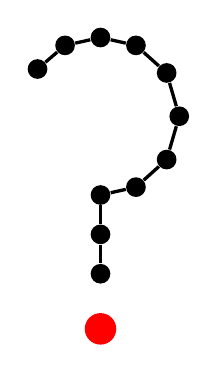
\begin{tikzpicture}[
        node/.style={circle, inner sep=0pt, fill=black, minimum size=2.5mm},
        node_c/.style={circle, inner sep=0pt, fill=red, minimum size=4mm}
        ]
        \node[node] at (-0.8, 0.6) (nm1) {};
        \node[node] at (-0.45, 0.9) (n0) {};
        \node[node] at (0, 1) (n1) {};
        \node[node] at (0.45, 0.9) (n2) {};
        \node[node] at (0.84, 0.55) (n3) {};
        \node[node] at (1, 0) (n4)  {};
        \node[node] at (0.84, -0.55) (n5) {};
        \node[node] at (0.45, -0.9) (n6) {};
        \node[node] at (0, -1) (n7) {};
        \node[node] at (0, -1.5) (n8) {};
        \node[node] at (0, -2) (n9) {};
        \node[node_c] at (0, -2.7) (n10) {};
        
        \draw[very thick]  (nm1) -- (n0);
        \draw[very thick]  (n0) -- (n1);
        \draw[very thick]  (n1) -- (n2);
        \draw[very thick]  (n2) -- (n3);
        \draw[very thick]  (n3) -- (n4);
        \draw[very thick]  (n4) -- (n5);
        \draw[very thick]  (n5) -- (n6);
        \draw[very thick]  (n6) -- (n7);
        \draw[very thick]  (n7) -- (n8);
        \draw[very thick]  (n8) -- (n9);
    \end{tikzpicture}
\end{figure}